\documentclass[11pt,a4paper]{article}
\usepackage[margin=24mm]{geometry}
\usepackage{tikz}
\title{Query-based hypergraph checks}
\date{Created 2026-09-29 12:40 CEST}
\begin{document}
\maketitle
\paragraph{Scope and estimate.} Add reusable match-count assertions to the existing
QueryEngine and apply named structural checks to the adversarial grid before any
search or export. Estimated 15--25 minutes for focused implementation, negative
fixtures, remote static validation and reporting. No simulation or new campaign.
\paragraph{Ownership.} Core remains the compiler and canonical IR owner. Query owns
predicate semantics and assertion evaluation; the example owns the grid-specific
rules. Graph keeps reachability/path search; HySTL keeps temporal monitoring.
No parser, solver, canonical model or temporal logic is reimplemented.
\paragraph{Files.} Query: src/checks.rs, src/lib.rs, src/predicate.rs,
src/engine.rs. Formats: examples/adversarial\_grid.rs and
data/adversarial\_grid\_queries.hymeko. This plan's tex/pdf/tikz/mmd files,
reports/2026-09-29-query-contracts.md and its verification artifacts.
\paragraph{API.} QueryEngine::check\_query evaluates a NamedQuery against an
Exactly/AtLeast/AtMost match expectation and returns the total count, pass/fail,
and a bounded sample of canonical DeclIds. EffectiveChildValue explicitly uses
the existing effective-field API, preserving direct ChildValue semantics.
Neutral-reference predicates must match only neutral signs; HasRef still matches
any sign. The grid example adds a static --check FILE command and query receipts.
\paragraph{Tests.} Exact/minimum/maximum counts, missing required matches, bounded
witnesses, effective inherited fields/local overrides and signed-reference
distinctions. Domain negative fixtures: a move to a wall, a non-cell reference,
invalid cell bounds, and successful original grids. Compile one saved nightly
world and run static checks on Amaterasu; no rollout is needed for this change.
\paragraph{Budget and risks.} Evaluation scans the existing query iterator; no
materialized graph or unbounded result vector. Witness memory is limited by the
caller. Retain existing 16x16, 1000-proposal and 300-second campaign caps. A query
assertion is not a proof of reachability or algorithm equivalence. Metadata
uniqueness, integer checks and geometry comparisons remain explicit domain checks.
\paragraph{State and rollback.} Reuse the current checkout and preserve all prior
evening-work changes. Fetch succeeded, HEAD equals upstream. No dependencies,
CORE.YAML files, branch switches, commits or pushes. Revert only this task's named
changes if needed. Local unit tests plus remote static replay, then archive the report.
\begin{center}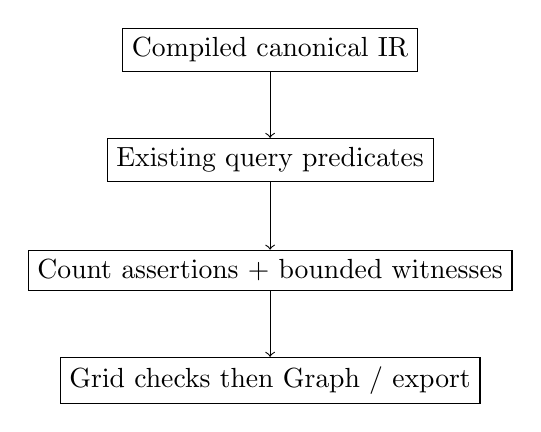
\begin{tikzpicture}[every node/.style={draw,align=center}]
\node (ir) at (0,0) {Compiled canonical IR};
\node (q) at (0,-1.4) {Existing query predicates};
\node (c) at (0,-2.8) {Count assertions + bounded witnesses};
\node (d) at (0,-4.2) {Grid checks then Graph / export};
\draw[->] (ir)--(q);\draw[->] (q)--(c);\draw[->] (c)--(d);
\end{tikzpicture}
\end{center}
\end{document}
